\section{Systembeskrivelse}
På Ingeniørhøjskolen Aarhus Universitet forefindes en AeroQuad Cyclone ARF Quadrocopter. 
Målet med projektet er, at omdanne quadrocopteren til en autonom overvågningsdrone.

Bruger skal kunne tilgå dronen via en webapplikation, som skal fungere som en grafisk brugerflade mellem bruger og drone. Via webapplikationen skal bruger blandt andet kunne lave opsætning til nye flyvninger, se billeder og flyverute fra tidligere flyvninger. 

Ved opsætning til ny flyvning vælger bruger en række GPS positioner som dronen skal flyve til. Desuden skal bruger vælge hvorvidt der skal tages billeder ved de valgte GPS positioner. 

Til enhver tid, skal al kommunikation mellem webapplikation og drone foregå via mobil netværk - hovedsageligt 3G. Da dronen skal flyve autonomt, er det vigtigt den kan orientere sig på egen hånd. Derfor er den udstyret med GPS, afstands sensorer og kompas.


\section{Systemoversigt}
Nederst til højre på systemskitsen ses et device med internet adgang. Dette devices bruges af bruger til at tilgå webapplikation, hvor opsætning af ny flyvning ordnes. Når en bruger har lavet indstillinger til ny flyvning, overføres opsætningen via internettet til dronen.
 
Via kommunikation med GPS satellitter finder dronen frem til egen position og hvilken retning den skal flyve i. Under flyvningen kan tage dronen billeder, som via nettet overføres til en database der er tilknyttet webapplikationen.

\vspace{-5pt}
%Systemskitse
\begin{figure}[H]
\centering
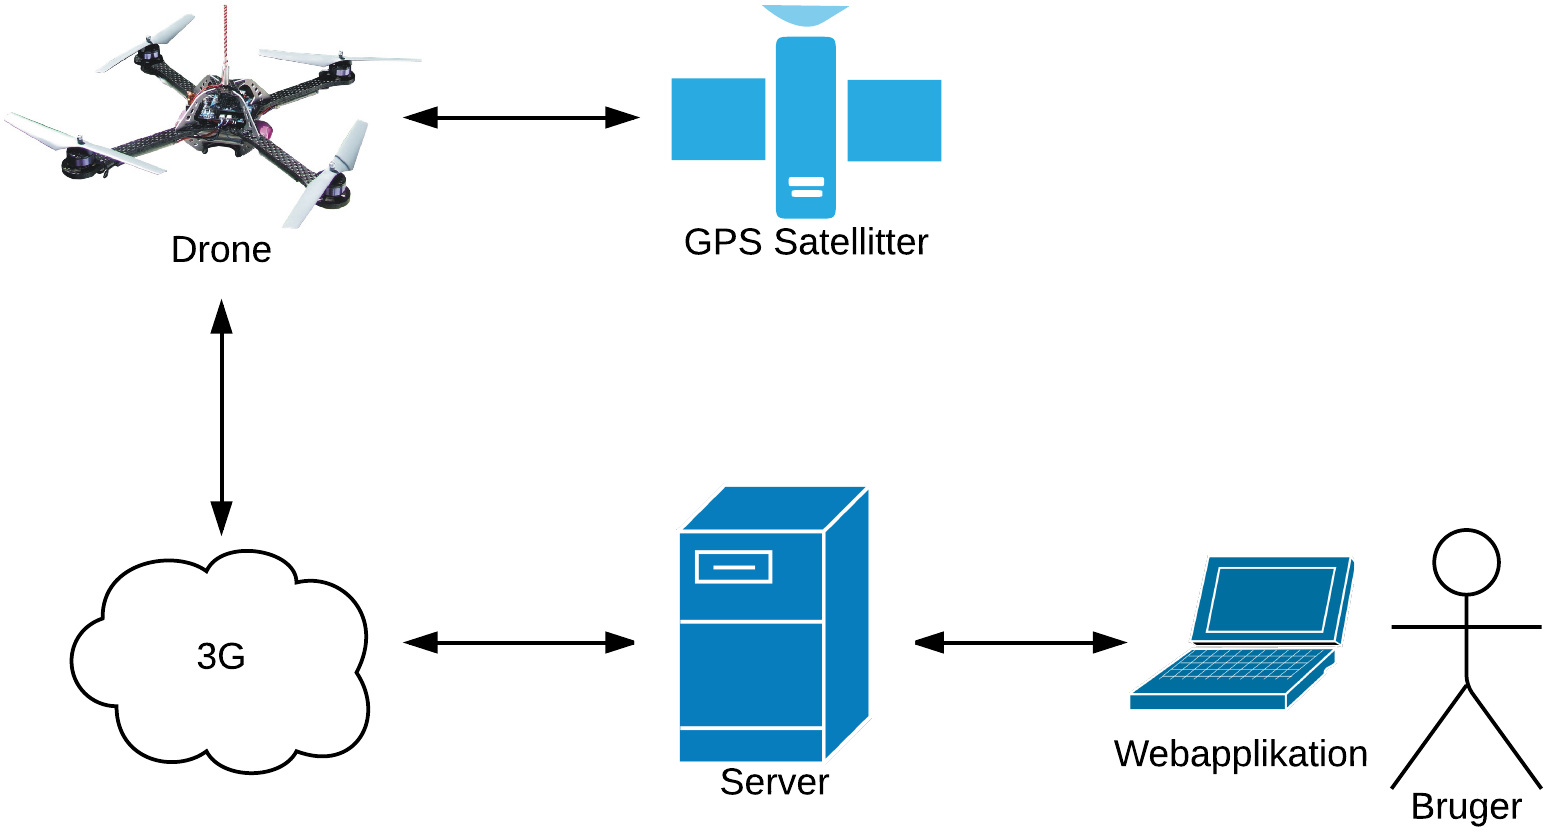
\includegraphics[width=1\textwidth]{Billeder/Projektbeskrivelse.png}
\vspace{-5pt}
\caption{Systemskitse}
\label{fig:Systemskitse}
\end{figure}